\chapter{SPICE Circuit Elements and Device Models}

\label{chap_spicecircuitelementsanddevicemodels_sceadm}

\section{SPICE Suffixes}
\label{subsec_sceadm_suffixes}

These suffixes are used in specifying parameter values for elements.

\begin{tabular}{lll} 
\textit{suffix} & \textit{name} & \textit{magnitude} \\ \hline \\ \vspace{-0.8\parskip}
a & atto- & $10^{-18}$ \\
f & femto- & $10^{-15}$ \\
p & pico- & $10^{-12}$ \\
n & nano- & $10^{-9}$ \\
u & micro- & $10^{-6}$ \\
m & milli- & $10^{-3}$ \\
k & kilo- & $10^{3}$ \\
meg & mega- & $10^{6}$ \\
g & giga- & $10^{9}$ \\
t & tera- & $10^{12}$ \\
\end{tabular}

\clearpage

\section{SPICE Element Identifiers}
\label{subsec_sceadm_elementidentifiers}

The SPICE netlist line for each type of circuit element must start with a specific character.  Here we list the characters all together; examples are presented throughout the rest of this chapter for each element type.

\begin{tabular}{lp{14cm}}
\textit{character} & \textit{element type}\\ \hline \\ \vspace{-0.8\parskip}
\texttt{R} & Resistors (Section \ref{subsec_sceadm_resistors}) \\
\texttt{C} & Capacitors (Section \ref{subsec_sceadm_capacitors}) \\
\texttt{L} & Inductors (Section \ref{subsec_sceadm_inductors}) \\
\texttt{K} & Coupled Inductors (Section \ref{subsec_sceadm_coupledinductors}) \\
\texttt{V} & Independent Voltage Sources (Section \ref{subsec_sceadm_independentsources}) \\
\texttt{I} & Independent Current Sources (Section \ref{subsec_sceadm_independentsources}) \\
\texttt{G} & Voltage-Controlled Current Sources (Section \ref{subsec_sceadm_lineardependentsources}) \\
\texttt{E} & Voltage-Controlled Voltage Sources (Section \ref{subsec_sceadm_lineardependentsources}) \\
\texttt{F} & Current-Controlled Current Sources (Section \ref{subsec_sceadm_lineardependentsources}) \\
\texttt{H} & Current-Controlled Voltage Sources (Section \ref{subsec_sceadm_lineardependentsources}) \\ 
\texttt{B} & Nonlinear Dependent (Behavioral) Sources (Section \ref{subsec_sceadm_behavioralsources}) \\
\texttt{D} & Diodes (Section \ref{subsec_sceadm_diodes}) \\
\texttt{Q} & BJTs (Section \ref{subsec_sceadm_bjts}) \\
\texttt{M} & MOSFETs (Section \ref{subsec_sceadm_mosfets}) \\
\texttt{Z} & MESFETs (Section \ref{subsec_sceadm_otheractiveelements}) \\
\texttt{J} & JFETs (Section \ref{subsec_sceadm_otheractiveelements}) \\
\texttt{S, W} & Switches (Section \ref{subsec_sceadm_switches}) \\
\texttt{T} & Transmission Lines (Section \ref{subsec_sceadm_transmissionlines}) \\

\end{tabular}

\section{Passive Elements}
\label{sec_sceadm_passiveelements}

\newpage
\subsection{Resistors}
\label{subsec_sceadm_resistors}

\textbf{\textit{Syntax:}}

\spicesyntax{\begin{tabular}{ll}
RXX & [N+] [N-] [VAL] [INLINE PARAMS]
\end{tabular}
}

\mymarginnote{Inline params\\are optional}

\begin{longtable}{l l}
\textit{parameter} & \textit{description} \\ \hline \\ \vspace{-0.8\parskip}
\texttt{[N+]} & Positive node/net \\
\texttt{[N-]} & Negative node/net \\
\texttt{[VAL]} & Resistance \\
\texttt{[INLINE PARAMS]} & \begin{tabular}{lp{5.5cm}p{5cm}}\textit{Inline parameters :}\\ 
																					{\small m : Current multiplication factor} \\ 
																					{\small ac : AC value} \\
																					{\small scale : Current scale factor} \\
																					{\small temp :  Temperature} \\
																					{\small dtemp : Temperature difference with ambient} \\
																					{\small tc1 : Linear temperature coefficient} \\
																					{\small tc2 : Quadratic temperature coefficient} \\
																					{\small noisy : Noise on/off}\end{tabular} 
\end{longtable}

\textbf{\textit{Schematics Editor Library:}}

Analog

\textbf{\textit{Schematics Editor Symbol:}}

\begin{figure}[htb]
  \begin{center}
    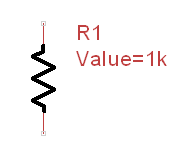
\includegraphics[width=0.15\textwidth]{./pics/SpiceEl/Resistor.png}
  \end{center}
	%\caption{Resistor symbol}
\end{figure}

\textbf{\textit{Schematics Editor Option:}}

"\textsf{Value}" is for assigning an alphanumeric number to \texttt{[VAL]}

\textbf{\textit{Examples:}}

\begin{longtable}{l l}
\textit{statement} & \textit{explanation} \\ \hline \\ \vspace{-0.8\parskip} 
\begin{minipage}{15em}\texttt{r1 1 0 1K}\end{minipage}  
& 
\begin{minipage}{15em}{\small Insert resistor r1, with resistance 1K$\Omega$, between nets 1 and 0}\end{minipage}  \\ \\ 
\begin{minipage}{15em}\texttt{r1 1 0 1K m=2 scale=3}\end{minipage}  
& 
\begin{minipage}{15em}{\small Insert resistor r1, with resistance 1K$\Omega \times \frac{3}{2}$, between nets 1 and 0}\end{minipage} 
\end{longtable}

\textbf{\textit{Remarks:}}

"\textsf{Value}" can be set to a model as described next by the alternative syntax. These alternatives can be used by editing the netlist using the netlist editor.
\newline\noindent
{\color{darkgray}
\textbf{\textit{Alternative Syntax 1:}}

\spicesyntax{\begin{tabular}{l}
RXX [N+] [N-] [VAL] [MODEL] [INLINE PARAMS] \\
.MODEL [MODEL] R [MODEL PARAMS]
\end{tabular}
}

\begin{longtable}{l l}
\textit{parameter} & \textit{description} \\ \hline \\ \vspace{-0.8\parskip}
\texttt{[N+]} & Positive node/net \\
\texttt{[N-]} & Negative node/net \\
\texttt{[VAL]} & Resistance \\
\texttt{[MODEL]} & Resistor model defined by a .model statement \\
\texttt{[INLINE PARAMS]} & \begin{tabular}{lp{5.5cm}p{5cm}}\textit{Inline parameters :} \\ 
																					{\small m : Current multiplication factor} \\ 
																					{\small ac : AC value} \\
																					{\small scale : Current scale factor} \\
																					{\small temp :  Temperature} \\
																					{\small dtemp : Temperature difference with ambient} \\
																					{\small tc1 : Linear temperature coefficient} \\
																					{\small tc2 : Quadratic temperature coefficient} \\
																					{\small noisy : Noise on/off}\end{tabular} \\
\texttt{[MODEL PARAMS]} & \begin{tabular}{lp{5.5cm}p{5cm}}\textit{Model parameters :} \\ 
																					{\small m : Current multiplication factor} \\ 
																					{\small ac : AC value} \\
																					{\small scale : Current scale factor} \\
																					{\small temp :  Temperature} \\
																					{\small dtemp : Temperature difference with ambient} \\
																					{\small tc1 : Linear temperature coefficient} \\
																					{\small tc2 : Quadratic temperature coefficient} \\
																					{\small noisy : Noise on/off}\end{tabular}																					
\end{longtable}

\textbf{\textit{Example:}}

\begin{longtable}{l l}
\textit{statement} & \textit{explanation} \\ \hline \\ %\vspace{-0.1\parskip} 
			\begin{minipage}{15em}{\texttt{r1 1 0 1K res tc1=0.01}\\ 
			\texttt{.model res R m=2}}\end{minipage}
			& \begin{minipage}{15em}{{\small Insert resistor r1, with resistance 1K$\Omega \times \frac{1}{2}$, between nets 1 and 0}}\end{minipage} 
\end{longtable}

\inserttip{If it is specified for an instance, [INLINE PARAMS] override [MODEL PARAMS].} 

\textbf{\textit{Alternative Syntax 2: Semiconductor resistor}}

\spicesyntax{\begin{tabular}{l}
RXX [N+] [N-] [VAL] [MODEL] [INLINE PARAMS] \\
.MODEL [MODEL] R [MODEL PARAMS]
\end{tabular}
}

\begin{longtable}{l l}
\textit{parameter} & \textit{description} \\ \hline \\ \vspace{-0.8\parskip}
\texttt{[N+]} & Positive node/net \\
\texttt{[N-]} & Negative node/net \\
\texttt{[VAL]} & Resistance \\
\texttt{[MODEL]} & Resistor model defined by a .model statement \\
\texttt{[INLINE PARAMS]} & \begin{tabular}{lp{5.5cm}p{5cm}}\textit{Inline parameters :} \\ 
																					{\small l : Length} \\
																					{\small w : Width} \\
																					{\small m : Current multiplication factor} \\ 
																					{\small ac : AC value} \\
																					{\small scale : Current scale factor} \\
																					{\small temp :  Temperature} \\
																					{\small dtemp : Temperature difference with ambient} \\
																					{\small noisy : Noise on/off}\end{tabular} \\
\texttt{[MODEL PARAMS]} & \begin{tabular}{lp{5.5cm}p{5cm}}\textit{Model parameters :} \\ 
																					{\small tc1 : Linear temperature coefficient} \\
																					{\small tc2 : Quadratic temperature coefficient} \\
																					{\small rsh : Sheet resistance} \\
																					{\small defw : Default width} \\
																					{\small narrow : Width narrowing value} \\
																					{\small short : Length shortening value} \\
																					{\small tnom : Nominal temperature} \\
																					{\small kf : Flicker noise coefficient} \\
																					{\small af : Flicker noise exponent} \\
																					{\small r (res) : Default value} \\
																					\end{tabular}																			
\end{longtable}

\textbf{\textit{Example:}}

\begin{longtable}{l l}
\textit{statement} & \textit{explanation} \\ \hline \\ %\vspace{-0.8\parskip} 
		\begin{minipage}{15em}{\texttt{r1 1 0 res l=2u w=1u} \\
			\texttt{.model res R (rsh=10\\+narrow=0.1u short=0.05u)}}\end{minipage} 
			& \begin{minipage}{15em}{{\small Insert resistor r1, with resistance 10$\times\frac{2u-0.05u}{1u-0.1u}\Omega$, between nets 1 and 0}}\end{minipage} 
\end{longtable}

\inserttip{If [VAL] is specified, it will override resistance calculated using the geometrical effects.} 

\textbf{\textit{Remarks:}}

If resistance is not specified, but tc1 (default : 0), tc2 (default : 0), rsh (no default), short (default : 0), and narrow (default : 0) are specified, the semiconductor resistance is calculated using the circuit temperature T as follows:

\begin{eqnarray}
\rm{r} &=& \rm{r}_o\times(1+\rm{tc1}\times(\rm{T}-\rm{tnom})+\rm{tc2}\times(\rm{T}-\rm{tnom})^2) \nonumber\\
\rm{r}_o &=& \rm{rsh}\times\frac{\rm{l}-\rm{short}}{\rm{w}-\rm{narrow}}\nonumber
\end{eqnarray} 

\inserttip{If rsh or l are not specified, r is set to 1m$\Omega$.} 

\textbf{\textit{Alternative Syntax 3: Behavioral resistor}}

\spicesyntax{\begin{tabular}{ll}
RXX & [N+] [N-] R= [EXPRESSION] [INLINE PARAMS]
\end{tabular}
}

\begin{longtable}{l l}
\textit{parameter} & \textit{description} \\ \hline \\ \vspace{-0.8\parskip}
\texttt{[N+]} & Positive node/net \\
\texttt{[N-]} & Negative node/net \\
\texttt{[EXPRESSION]} & An equation or expression containing voltages or currents \\
\texttt{[INLINE PARAMS]} & \begin{tabular}{lp{5.5cm}p{5cm}}\textit{Inline parameters :} \\ 
																					{\small tc1 : Linear temperature coefficient} \\
																					{\small tc2 : Quadratic temperature coefficient} 
																					\end{tabular} 																	
\end{longtable}

\textbf{\textit{Example:}}

\begin{longtable}{l l}
\textit{statement} & \textit{explanation} \\ \hline \\ %\vspace{-0.8\parskip} 
		\begin{minipage}{15em}\texttt{r1 1 0 r={v(2)*0.1}}\end{minipage} 
			& \begin{minipage}{15em}{\small Insert resistor r1, with resistance v(2)$\times$0.1$\Omega$, between nets 1 and 0}\end{minipage} 
\end{longtable}
}

\inserttip{Expression needs to be enclosed with $\{...\}$ or '...'.} 

% CAPACITOR CAPACITOR
\newpage
\subsection{Capacitors}
\label{subsec_sceadm_capacitors}

\textbf{\textit{Syntax:}}

\spicesyntax{\begin{tabular}{ll}
CXX & [N+] [N-] [VAL] [INLINE PARAMS]
\end{tabular}
}

\begin{longtable}{l l}
\textit{parameter} & \textit{description} \\ \hline \\ \vspace{-0.8\parskip}
\texttt{[N+]} & Positive node/net \\
\texttt{[N-]} & Negative node/net \\
\texttt{[VAL]} & Capacitance \\
\texttt{[INLINE PARAMS]} & \begin{tabular}{lp{5.5cm}p{5cm}}\textit{Inline parameters :}\\ 
																					{\small m : Current multiplication factor} \\ 
																					{\small scale : Current scale factor} \\
																					{\small temp :  Temperature} \\
																					{\small dtemp : Temperature difference with ambient} \\
																					{\small tc1 : Linear temperature coefficient} \\
																					{\small tc2 : Quadratic temperature coefficient} \\
																					{\small ic : Initial condition} \\
																					{\small rser : Series resistance} \\
																					{\small lser : Series inductance} \\ 
																					{\small rpar : Parallel resistance} \\
																					{\small cpar : Parallel capacitance} \\
																					{\small rlshunt : Parallel resistance to lser} 
																					\end{tabular} 
\end{longtable}

\inserttip{rser, lser, rpar, cpar and rlshunt are incorporated for Ltspice compatibility.}

\textbf{\textit{Schematics Editor Library:}}

Analog

\textbf{\textit{Schematics Editor Symbol:}}

\begin{figure}[htb]
  \begin{center}
    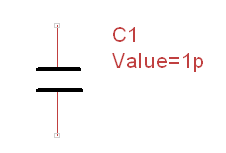
\includegraphics[width=0.15\textwidth]{./pics/SpiceEl/Capacitor.png}
  \end{center}
	%\caption{Resistor symbol}
\end{figure}

\textbf{\textit{Schematics Editor Option:}}

"\textsf{Value}" is for assigning an alphanumeric number to \texttt{[VAL]}

\textbf{\textit{Examples:}}

\begin{longtable}{l l}
\textit{statement} & \textit{explanation} \\ \hline \\ \vspace{-0.8\parskip} 
\begin{minipage}{15em}\texttt{c1 1 0 1p}\end{minipage} & 
\begin{minipage}{15em}{\small Insert capacitor c1, with capacitance 1pF, between nets 1 and 0}\end{minipage} \\
\begin{minipage}{15em}\texttt{c1 1 0 1K m=2 scale=3}\end{minipage} & 
\begin{minipage}{15em}{\small Insert capacitor c1, with capacitance 1pF $\times$2$\times$3, between nets 1 and 0}\end{minipage}
\end{longtable}

\textbf{\textit{Remarks:}}

"\textsf{Value}" can be set to a model as described next by the alternative syntax. These alternatives can be used by editing the netlist using the netlist editor.

\mymarginnote{Default gmin\\is 1e-12} 

\inserttip{CoolSPICE automatically inserts a resistor with resistance 1/gmin across each capacitor to increase stability.}




{\color{darkgray}
\textbf{\textit{Alternative Syntax 1:}}

\spicesyntax{\begin{tabular}{l}
CXX [N+] [N-] [VAL] [MODEL] [INLINE PARAMS] \\
.MODEL [MODEL] C [MODEL PARAMS]
\end{tabular}
}

\begin{longtable}{l l}
\textit{parameter} & \textit{description} \\ \hline \\ \vspace{-0.8\parskip}
\texttt{[N+]} & Positive node/net \\
\texttt{[N-]} & Negative node/net \\
\texttt{[VAL]} & Capacitance \\
\texttt{[MODEL]} & Capacitance model defined by a .model statement \\
\texttt{[INLINE PARAMS]} & \begin{tabular}{lp{5.5cm}p{5cm}}\textit{Inline parameters :} \\ 
																					{\small m : Current multiplication factor} \\ 
																					{\small scale : Current scale factor} \\
																					{\small temp :  Temperature} \\
																					{\small dtemp : Temperature difference with ambient} \\
																					{\small tc1 : Linear temperature coefficient} \\
																					{\small tc2 : Quadratic temperature coefficient} \\
																					{\small ic : Initial condition} \\
																					{\small rser : Series resistance} \\
																					{\small lser : Series inductance} \\ 
																					{\small rpar : Parallel resistance} \\
																					{\small cpar : Parallel capacitance} \\
																					{\small rlshunt : Parallel resistance to lser}																					\end{tabular} \\
\texttt{[MODEL PARAMS]} & \begin{tabular}{lp{5.5cm}p{5cm}}\textit{Model parameters :} \\ 
																					{\small cap : Capacitance} \\
																					{\small m : Current multiplication factor} \\ 
																					{\small scale : Current scale factor} \\
																					{\small temp :  Temperature} \\
																					{\small dtemp : Temperature difference with ambient} \\
																					{\small tc1 : Linear temperature coefficient} \\
																					{\small tc2 : Quadratic temperature coefficient} \\
																					{\small ic : Initial condition}\end{tabular}																					
\end{longtable}

\textbf{\textit{Example:}}

\begin{longtable}{l l}
\textit{statement} & \textit{explanation} \\ \hline \\ %\vspace{-0.1\parskip} 
			\begin{minipage}{15em}{\texttt{c1 1 0 1p cap tc1=0.01}\\ 
			\texttt{.model cap C m=2}}\end{minipage}
			& \begin{minipage}{15em}{{\small Insert capacitor c1, with capacitance 1pF $\times$2, between nets 1 and 0}}\end{minipage} 
\end{longtable}

\inserttip{.ic applies only if uic is used in conjunction with .tran.} 

\textbf{\textit{Alternative Syntax 2: Semiconductor capacitor}}

\spicesyntax{\begin{tabular}{l}
CXX [N+] [N-] [VAL] [MODEL] [INLINE PARAMS] \\
.MODEL [MODEL] C [MODEL PARAMS]
\end{tabular}
}

\begin{longtable}{l l}
\textit{parameter} & \textit{description} \\ \hline \\ \vspace{-0.8\parskip}
\texttt{[N+]} & Positive node/net \\
\texttt{[N-]} & Negative node/net \\
\texttt{[VAL]} & Capacitance \\
\texttt{[MODEL]} & Resistor model defined by a .model statement \\
\texttt{[INLINE PARAMS]} & \begin{tabular}{lp{5.5cm}p{5cm}}\textit{Inline parameters :} \\ 
																					{\small l : Length} \\
																					{\small w : Width} \\
																					{\small m : Current multiplication factor} \\ 
																					{\small scale : Current scale factor} \\
																					{\small temp :  Temperature} \\
																					{\small dtemp : Temperature difference with ambient} \\
																					{\small ic : Initial condition} \\
																					{\small rser : Series resistance} \\
																					{\small lser : Series inductance} \\ 
																					{\small rpar : Parallel resistance} \\
																					{\small cpar : Parallel capacitance} \\
																					{\small rlshunt : Parallel resistance to lser}
																					\end{tabular} \\
\texttt{[MODEL PARAMS]} & \begin{tabular}{lp{5.5cm}p{5cm}}\textit{Model parameters :} \\ 
																					{\small cap : Default value}  \\
																					{\small cj : Bottom/areal junction capacitance} \\
																					{\small cjsw : Sidewall/perimeter junction capacitance} \\
																					{\small defw : Default width} \\
																					{\small defl : Default length} \\
																					{\small defw : Default width} \\
																					{\small narrow : Width narrowing value} \\
																					{\small short : Length shortening value} \\
																					{\small tc1 : Linear temperature coefficient} \\
																					{\small tc2 : Quadratic temperature coefficient} \\
																					{\small tnom : Nominal temperature} \\
																					{\small di : Relative epsilon} \\
																					{\small thick : Dielectric thickness} \\
																					\end{tabular}																			
\end{longtable}

\textbf{\textit{Example:}}

\begin{longtable}{l l}
\textit{statement} & \textit{explanation} \\ \hline \\ %\vspace{-0.8\parskip} 
		\begin{minipage}{15em}{\texttt{c1 1 0 cap l=2u w=1u} \\
			\texttt{.model cap C (cj=1u cjsw=1p)}}\end{minipage} 
			& \begin{minipage}{15em}{{\small Insert capacitor c1, with capacitance 
			1uF/m$^{2}\times\rm{l}\times\rm{w}$ + 1pF/m $\times{2}\times\rm{l}\times\rm{w}$, between nets 1 and 0}}\end{minipage}  
\end{longtable}

\textbf{\textit{Remarks:}}

If cap is not specified, but tc1 (default : 0), tc2 (default : 0), thick (default : 0), short (default : 0), narrow (default : 0), and di (default : 3.9) are specified, the semiconductor capacitance is calculated using the circuit temperature T as follows:

\begin{eqnarray}
\rm{c} &=& \rm{c}_o\times(1+\rm{tc1}\times(\rm{T}-\rm{tnom})+\rm{tc2}\times(\rm{T}-\rm{tnom})^2) \nonumber\\
\rm{c}_o &=& \rm{cj}\times(\rm{l}-\rm{short}) + 2\times\rm{cjsw}\times(\rm{l}-\rm{short}+\rm{w}-\rm{narrow}) \nonumber\\
\rm{cj} &=& \frac{\rm{cj}\times\epsilon_o}{\rm{thick}}\nonumber
\end{eqnarray} 

\inserttip{If [VAL] is specified, it will override capacitance calculated using the geometrical effects.} 

\textbf{\textit{Alternative Syntax 3: Behavioral capacitor}}

\spicesyntax{\begin{tabular}{ll}
CXX & [N+] [N-] C= [EXPRESSION] [INLINE PARAMS]  
\end{tabular}
}

\begin{longtable}{l l}
\textit{parameter} & \textit{description} \\ \hline \\ \vspace{-0.8\parskip}
\texttt{[N+]} & Positive node/net \\
\texttt{[N-]} & Negative node/net \\
\texttt{[EXPRESSION]} & An equation or expression containing voltages or currents \\
\texttt{[INLINE PARAMS]} & \begin{tabular}{lp{5.5cm}p{5cm}}\textit{Inline parameters :} \\ 
																					{\small tc1 : Linear temperature coefficient} \\
																					{\small tc2 : Quadratic temperature coefficient} \\
																					{\small rser : Series resistance} \\
																					{\small lser : Series inductance} \\ 
																					{\small rpar : Parallel resistance} \\
																					{\small cpar : Parallel capacitance} \\
																					{\small rlshunt : Parallel resistance to lser}
																					\end{tabular}  																	
\end{longtable}

\textbf{\textit{Example:}}

\begin{longtable}{l l}
\textit{statement} & \textit{explanation} \\ \hline \\ %\vspace{-0.8\parskip} 
		\begin{minipage}{15em}\texttt{c1 1 0 c={v(2)*0.1}}\end{minipage} 
			& \begin{minipage}{15em}{\small Insert capacitor c1, with capacitance v(2)$\times$0.1F, between nets 1 and 0}\end{minipage} 
\end{longtable}
}

% INDUCTOR INDUCTOR
\newpage
\subsection{Inductors}
\label{subsec_sceadm_inductors}

\textbf{\textit{Syntax:}}

\spicesyntax{\begin{tabular}{ll}
LXX & [N+] [N-] [VAL] [INLINE PARAMS]
\end{tabular}
}

\begin{longtable}{l l}
\textit{parameter} & \textit{description} \\ \hline \\ \vspace{-0.8\parskip}
\texttt{[N+]} & Positive node/net \\
\texttt{[N-]} & Negative node/net \\
\texttt{[VAL]} & Inductance \\
\texttt{[INLINE PARAMS]} & \begin{tabular}{lp{5.5cm}p{5cm}}\textit{Inline parameters :}\\
																					{\small nt : Number of turns} \\ 
																					{\small m : Current multiplication factor} \\ 
																					{\small scale : Current scale factor} \\
																					{\small temp :  Temperature} \\
																					{\small dtemp : Temperature difference with ambient} \\
																					{\small tc1 : Linear temperature coefficient} \\
																					{\small tc2 : Quadratic temperature coefficient} \\
																					{\small ic : Initial condition} \\
																					{\small rser : Series resistance} \\
																					{\small rpar : Parallel resistance} \\
																					{\small cpar : Parallel capacitance} 
																					\end{tabular} 
\end{longtable}

\inserttip{rser, rpar, and cpar are incorporated for Ltspice compatibility.}

\textbf{\textit{Schematics Editor Library:}}

Analog

\textbf{\textit{Schematics Editor Symbol:}}

\begin{figure}[htb]
  \begin{center}
    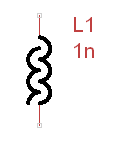
\includegraphics[width=0.125\textwidth]{./pics/SpiceEl/Inductor.png}
  \end{center}
	%\caption{Resistor symbol}
\end{figure}

\textbf{\textit{Schematics Editor Option:}}

"\textsf{Value}" is for assigning an alphanumeric number to \texttt{[VAL]}
\newpage
\textbf{\textit{Examples:}}

\begin{longtable}{l l}
\textit{statement} & \textit{explanation} \\ \hline \\ \vspace{-0.8\parskip} 
\begin{minipage}{15em}\texttt{l1 1 0 1n}\end{minipage} & 
\begin{minipage}{15em}{\small Insert inductor l1, with inductance 1nH, between nets 1 and 0}\end{minipage} \\ \\
\begin{minipage}{15em}\texttt{l1 1 0 1n m=2}\end{minipage} & 
\begin{minipage}{15em}{\small Insert inductor l1, with inductance 1nF $\times$2, between nets 1 and 0}\end{minipage}
\end{longtable}

\textbf{\textit{Remarks:}}

"\textsf{Value}" can be set to a model as described next by the alternative syntax. These alternatives can be used by editing the netlist using the netlist editor.

\mymarginnote{Default gmin\\is 1e-12} 

\inserttip{CoolSPICE automatically inserts a resistor with resistance 1/gmin across each inductor to increase stability.}

\inserttip{CoolSPICE automatically inserts a 1 m$\Omega$ resistor in series with each inductor to increase stability. This can be disabled globally or locally.}


{\color{darkgray}
\textbf{\textit{Alternative Syntax 1:}}

\spicesyntax{\begin{tabular}{l}
LXX [N+] [N-] [VAL] [MODEL] [INLINE PARAMS] \\
.MODEL [MODEL] L [MODEL PARAMS]
\end{tabular}
}

\begin{longtable}{l l}
\textit{parameter} & \textit{description} \\ \hline \\ \vspace{-0.8\parskip}
\texttt{[N+]} & Positive node/net \\
\texttt{[N-]} & Negative node/net \\
\texttt{[VAL]} & Capacitance \\
\texttt{[MODEL]} & Capacitance model defined by a .model statement \\
\texttt{[INLINE PARAMS]} & \begin{tabular}{lp{5.5cm}p{5cm}}\textit{Inline parameters :} \\ 
																					{\small m : Current multiplication factor} \\ 
																					{\small scale : Current scale factor} \\
																					{\small nt : Number of turns} \\
																					{\small temp :  Temperature} \\
																					{\small dtemp : Temperature difference with ambient} \\
																					{\small tc1 : Linear temperature coefficient} \\
																					{\small tc2 : Quadratic temperature coefficient} \\
																					{\small ic : Initial condition} \\
																					{\small rser : Series resistance} \\
																					{\small rpar : Parallel resistance} \\
																					{\small cpar : Parallel capacitance} 																					\end{tabular} \\
\texttt{[MODEL PARAMS]} & \begin{tabular}{lp{5.5cm}p{5cm}}\textit{Model parameters :} \\ 
																					{\small ind : Capacitance} \\
																					{\small csect : Cross section} \\ 
																					{\small length : Length} \\
																					{\small tc1 : Linear temperature coefficient} \\
																					{\small tc2 : Quadratic temperature coefficient} \\
																					{\small tnom :  Nominal temperature} \\
																					{\small nt : Number of turns} \\
																					{\small mu : Relative $\mu$} \\																					  
																					\end{tabular}																					
\end{longtable}

\textbf{\textit{Example:}}

\begin{longtable}{l l}
\textit{statement} & \textit{explanation} \\ \hline \\ %\vspace{-0.1\parskip} 
			\begin{minipage}{15em}{\texttt{l1 1 0 1n myind tc1=0.01}\\ 
			\texttt{.model myind L m=2}}\end{minipage}
			& \begin{minipage}{15em}
			{{\small Insert inductor l1, with inductance 1nH $\times$0.5, between nets 1 and 0}}
			\end{minipage}
				
\end{longtable}

\inserttip{.ic applies only if uic is used in conjunction with .tran.} 

\textbf{\textit{Remarks:}}

If ind is not specified, but tc1 (default : 0), tc2 (default : 0), nt (default : 0), csect (default : 0), mu (default : 1), and length (default : 0) are specified, the inductance is calculated using the circuit temperature T as follows:

\begin{eqnarray}
\rm{l} &=& \rm{l}_o\times(1+\rm{tc1}\times(\rm{T}-\rm{tnom})+\rm{tc2}\times(\rm{T}-\rm{tnom})^2) \nonumber\\
\rm{l}_o &=& \frac{\rm{mu}\times\mu_o\times\rm{nt}^2\times\rm{csect}}{\rm{length}}\nonumber
\end{eqnarray} 

\inserttip{If [VAL] is specified, it will override inductance calculated using the geometrical effects.} 

\textbf{\textit{Alternative Syntax 3: Behavioral inductor}}

\spicesyntax{\begin{tabular}{ll}
LXX & [N+] [N-] C= [EXPRESSION] [INLINE PARAMS]  
\end{tabular}
}

\begin{longtable}{l l}
\textit{parameter} & \textit{description} \\ \hline \\ \vspace{-0.8\parskip}
\texttt{[N+]} & Positive node/net \\
\texttt{[N-]} & Negative node/net \\
\texttt{[EXPRESSION]} & An equation or expression containing voltages or currents \\
\texttt{[INLINE PARAMS]} & \begin{tabular}{lp{5.5cm}p{5cm}}\textit{Inline parameters :} \\ 
																					{\small tc1 : Linear temperature coefficient} \\
																					{\small tc2 : Quadratic temperature coefficient} \\
																					{\small rser : Series resistance} \\
																					{\small rpar : Parallel resistance} \\
																					{\small cpar : Parallel capacitance} 
																					\end{tabular}  																	
\end{longtable}

\textbf{\textit{Example:}}

\begin{longtable}{l l}
\textit{statement} & \textit{explanation} \\ \hline \\ %\vspace{-0.8\parskip} 
		\begin{minipage}{15em}\texttt{l1 1 0 l={v(2)*0.1}}\end{minipage} 
			& \begin{minipage}{15em}{\small Insert inductor l1, with inductance v(2)$\times$0.1H, between nets 1 and 0}\end{minipage} 
\end{longtable}
}


% COUPLED INDUCTOR COUPLED INDUCTOR
\newpage
\subsection{Coupled Inductors}
\label{subsec_sceadm_coupledinductors}

\textbf{\textit{Syntax:}}

\spicesyntax{\begin{tabular}{ll}
KXX & [LYY] [LZZ] [VAL] 
\end{tabular}
}

\begin{longtable}{l l}
\textit{parameter} & \textit{description} \\ \hline \\ \vspace{-0.8\parskip}
\texttt{[LYY]} & First of the coupled inductor \\
\texttt{[LZZ]} & Second of the coupled inductor \\
\texttt{[VAL]} & Coupling value \\ 
\end{longtable}

\inserttip{Coupling value has to be between 0 and 1.}

\textbf{\textit{Schematics Editor Library:}}

Analog

\textbf{\textit{Schematics Editor Symbol:}}

\begin{figure}[htb]
  \begin{center}
    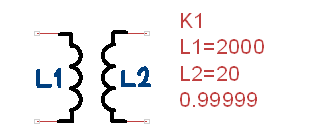
\includegraphics[height=0.08\textheight]{./pics/SpiceEl/CInductor.png}
  \end{center}
	%\caption{Resistor symbol}
\end{figure}

\textbf{\textit{Schematics Editor Option:}}

"\textsf{Value}" is for assigning an alphanumeric number to \texttt{[VAL]}

\textbf{\textit{Examples:}}

\begin{longtable}{l l}
\textit{statement} & \textit{explanation} \\ \hline \\ \vspace{-0.8\parskip} 
\begin{minipage}{15em}\texttt{k1 l1 l2 0.99}\end{minipage} & 
\begin{minipage}{15em}{\small Insert coupled inductor k1, with coupling 0.99, between nets 1 and 0}\end{minipage} \\
\end{longtable}



\newpage
\section{Sources}
\label{sec_sceadm_sources}

\subsection{Independent Sources}
\label{subsec_sceadm_independentsources}

\textbf{\textit{Syntax:}}

\spicesyntax{\begin{tabular}{ll}
VXX & [N+] [N-] [DC] [AC] [DISTOF1] [DISTOF2] [FUNCTION]\\
IXX & [N+] [N-] [DC] [AC] [DISTOF1] [DISTOF2] [FUNCTION]
\end{tabular}
}


\begin{longtable}{l l}
\textit{parameter} & \textit{description} \\ \hline \\ \vspace{-0.8\parskip}
\texttt{[N+]} & Positive node/net \\
\texttt{[N-]} & Negative node/net \\
\texttt{[DC]} & DC offset during a DC or transient run \\
\texttt{[AC]} & \begin{tabular}{lp{5.5cm}p{5cm}}\textit{AC parameters :}\\ 
																					{\small ACMAG : AC magnitude} \\ 
																					{\small ACPHASE : AC phase} \\
																					\end{tabular} \\
\texttt{[DISTOF1]} & \begin{tabular}{lp{5.5cm}p{5cm}}\textit{1$^{st}$ distortion parameters :}\\ 
																					{\small F1MAG : Distortion frequency} \\ 
																					{\small F1PHASE : Distortion phase} \\
																					\end{tabular} \\	
\texttt{[DISTOF2]} & \begin{tabular}{lp{5.5cm}p{5cm}}\textit{2$^{nd}$ distortion parameters :}\\ 
																					{\small F2MAG : Distortion frequency} \\ 
																					{\small F2PHASE : Distortion phase} \\
																					\end{tabular} \\
\texttt{[FUNCTION]} & \begin{tabular}{lp{5.5cm}p{5cm}}\textit{Temporal functions :}\\ 
																					{\small Pulse} \\ 
																					{\small Exponential} \\
																					{\small Sinusoidal} \\
																					{\small Piecewise linear} \\
																					{\small Single frequency FM} \\
																					{\small AM} \\
																					{\small Transient noise} \\
																					{\small Random voltages or currents} \\
																					\end{tabular}													
\end{longtable}

\textbf{\textit{Schematics Editor Library:}}

Analog

\textbf{\textit{Schematics Editor Symbol:}}

\begin{figure}[htb]
  \begin{center}
    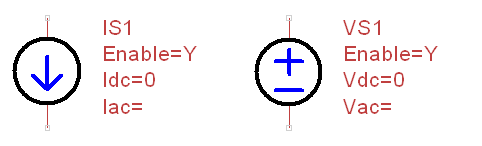
\includegraphics[height=0.08\textheight]{./pics/SpiceEl/IV.png}
  \end{center}
\end{figure}

\textbf{\textit{Schematics Editor Option:}}

"\textsf{Idc / Vdc}"  is for assigning an alphanumeric value to \texttt{[DC]}. "\textsf{Iac / Vac}"  is for assigning an alphanumeric value to \texttt{[AC]}.

\textbf{\textit{Examples:}}

\begin{longtable}{l l}
\textit{statement} & \textit{explanation} \\ \hline \\ \vspace{-0.8\parskip} 
\begin{minipage}{15em}\texttt{v1 1 0 1 0.1}\end{minipage}  
& 
\begin{minipage}{15em}{\small Insert voltage source v1, with 1V DC and 0.1V AC, between nets 1 and 0}\end{minipage}  \\ \\ 
\begin{minipage}{15em}\texttt{i1 1 0 1 0.1}\end{minipage}  
& 
\begin{minipage}{15em}{\small Insert current source i1, with 1V DC and 0.1V AC, between nets 1 and 0}\end{minipage}  \\ \\ 
\begin{minipage}{15em}\texttt{i1 1 0 sin(0 1 1meg)}\end{minipage}  
& 
\begin{minipage}{15em}{\small Insert sinusoidal current source i1, with 1V magnitude and 1MHz frequency, between nets 1 and 0}\end{minipage}
\end{longtable}

\textbf{\textit{Pulse Waveform Syntax:}}

\spicesyntax{\begin{tabular}{l}
PULSE ( [V1] [V2] [TD] [TR] [TF] [PW] [PER] )
\end{tabular}
}

\begin{longtable}{l l}
\textit{parameter} & \textit{description} \\ \hline \\ \vspace{-0.8\parskip}
\texttt{[V1]} & Initial pulse value \\
\texttt{[V2]} & Pulsed value \\
\texttt{[TD]} & Delay time \\
\texttt{[TR]} & Rise time \\
\texttt{[TF]} & Fall time \\
\texttt{[PW]} & Pulse width \\
\texttt{[PER]} & Period
\end{longtable}

\textbf{\textit{Closed Form:}}

  \[
    V(t)=\left\{
                \begin{array}{l l}
                  \rm{V1} \hspace{1.9in} \rm{if\ }0\leq t<\rm{TD}\\
                  \rm{V1}+(\rm{V2}-\rm{V1})\frac{t-\rm{TD}}{\rm{TR}}\hspace{0.55in}\rm{\ if\ TD}\leq t<\rm{TD}+\rm{TR}\\
									\rm{V2} \hspace{1.9in} \rm{if\ TD}+\rm{TR}\leq t<\rm{TD}+\rm{TR}+\rm{PW}\\
                  \rm{V2}+(\rm{V1}-\rm{V2})\frac{t-\rm{TD}-\rm{TR}-\rm{PW}}{\rm{TF}}\rm{\ if\ }\rm{TD}+\rm{TR}+\rm{PW}\leq t<\rm{TD}+\rm{TR}+\rm{PW}+\rm{TF}\\
									\rm{V1} \hspace{1.9in} \rm{if\ }\rm{TD}+\rm{TR}+\rm{PW}+\rm{TF}\leq t<\rm{PER}
                \end{array}
              \right.
  \]

\textbf{\textit{Examples:}}

\begin{longtable}{l l}
\textit{statement} & \textit{explanation} \\ \hline \\ \vspace{-0.8\parskip} 
\begin{minipage}{15em}\texttt{v1 1 0 pulse(0 1 1n 2n 3n 20n 50n)}\end{minipage}  
& 
\begin{minipage}{15em}{\small Insert pulsed voltage source v1 between nets 1 and 0. Pulse source generates a pulse train. The start is delayed by 1ns. The initial DC value is set to the t=0 value. v(1) voltage changes from 0 to 1V between t=1ns and t=3ns. It stays at 1V between t=3ns and t=23ns. It then falls from 1V to 0 between t=23ns and t=26ns. It stays at 0 until t=51ns. 1ns shifted (delayed canceled) version of this initial waveform repeats itself until simulation end time.}\end{minipage}  
\end{longtable}

\textbf{\textit{Sinusoidal Waveform Syntax:}}

\spicesyntax{\begin{tabular}{l}
SIN ( [VO] [VA] [FREQ] [TD] [THETA] )
\end{tabular}
}

\begin{longtable}{l l}
\textit{parameter} & \textit{description} \\ \hline \\ \vspace{-0.8\parskip}
\texttt{[VO]} & Voltage offset \\
\texttt{[VA]} & Sinusoidal wave amplitude \\
\texttt{[FREQ]} & Sinusoidal wave frequency \\
\texttt{[TD]} & Delay time \\
\texttt{[THETA]} & Damping factor 
\end{longtable}

\textbf{\textit{Closed Form:}}

  \[
    V(t)=\left\{
                \begin{array}{l l}
                  \rm{VO} \hspace{3.85in} \rm{if\ }0\leq t<\rm{TD}\\
                  \rm{VO}+\rm{VA}\exp(-(t-\rm{TD})\rm{THETA})\sin(2\pi\rm{FREQ}(t-\rm{TD})) \rm{\ if\ TD}\leq t<\rm{TSTOP}\\
                \end{array}
              \right.
  \]

\textbf{\textit{Examples:}}

\begin{longtable}{l l}
\textit{statement} & \textit{explanation} \\ \hline \\ \vspace{-0.8\parskip} 
\begin{minipage}{15em}\texttt{v1 1 0 sin(0 1 1meg 0 0)}\end{minipage}  
& 
\begin{minipage}{15em}{\small Insert sinusoidal voltage source v1 between nets 1 and 0. The initial DC value is set to the t=0 value. v(1) voltage sinusoidally changes from -1V to 1V with 1MHz frequency.}\end{minipage}  
\end{longtable}

\textbf{\textit{Exponential Waveform Syntax:}}

\spicesyntax{\begin{tabular}{l}
EXP ( [V1] [V2] [TD1] [TAU1] [TD2] [TAU2] )
\end{tabular}
}

\begin{longtable}{l l}
\textit{parameter} & \textit{description} \\ \hline \\ \vspace{-0.8\parskip}
\texttt{[V1]} & Initial value \\
\texttt{[V2]} & Pulsed value \\
\texttt{[TD1]} & Rise delay \\
\texttt{[TAU1]} & Rise time constant \\
\texttt{[TD2]} & Fall delay \\
\texttt{[TAU2]} & Fall time constant
\end{longtable}

\textbf{\textit{Closed Form:}}

  \[
    V(t)=\left\{
                \begin{array}{l l}
                  \rm{V1} \hspace{3.8in} \rm{if\ }0\leq t<\rm{TD1}\\
                  \rm{V1}+(\rm{V2}-\rm{V1})(1-e^{-\frac{t-\rm{TD}}{\rm{TAU1}}})\hspace{1.9in}\rm{\ if\ TD1}\leq t<\rm{TD2}\\
									\rm{V1}+(\rm{V2}-\rm{V1})(1-e^{-\frac{t-\rm{TD1}}{\rm{TAU1}}})+(\rm{V1}-\rm{V2})(1-e^{-\frac{t-\rm{TD2}}{\rm{TAU2}}})\rm{\ if\ TD2}\leq t<\rm{TSTOP}
                \end{array}
              \right.
  \]

\textbf{\textit{Examples:}}

\begin{longtable}{l l}
\textit{statement} & \textit{explanation} \\ \hline \\ \vspace{-0.8\parskip} 
\begin{minipage}{15em}\texttt{v1 1 0 exp(0 1 0 6n 20n 6n)}\end{minipage}  
& 
\begin{minipage}{15em}{\small Insert exponential voltage source v1 between nets 1 and 0. The initial DC value is set to the t=0 value.}\end{minipage}  
\end{longtable}

\textbf{\textit{Piecewise Linear Waveform Syntax:}}

\spicesyntax{\begin{tabular}{l}
PWL ( [T1] [V1] [T2] [V2] [T3] [V3] [T4] [V4] ... ) [INLINE PARAMS]
\end{tabular}
}

\begin{longtable}{l l}
\textit{parameter} & \textit{description} \\ \hline \\ \vspace{-0.8\parskip}
\texttt{[V1] [V2] ...} & Voltage points \\
\texttt{[T1] [T2] ...} & Time points \\
\texttt{[INLINE PARAMS]} & \begin{tabular}{lp{5.5cm}p{5cm}}\textit{Inline parameters :}\\ 
																					{\small r : Repeat interval from r to the last [TN]} \\
																					{\small td : Delay}
																					\end{tabular}  
\end{longtable}

\textbf{\textit{FM Waveform Syntax:}}

\spicesyntax{\begin{tabular}{l}
SFFM ( [VO] [VA] [MDI] [FS] )
\end{tabular}
}

\begin{longtable}{l l}
\textit{parameter} & \textit{description} \\ \hline \\ \vspace{-0.8\parskip}
\texttt{[VO]} & Offset \\
\texttt{[VA]} & Amplitude \\
\texttt{[FC]} & Carrier frequency \\
\texttt{[MDI]} & Modulation \\
\texttt{[FS]} & Signal frequency 
\end{longtable}

\textbf{\textit{Closed Form:}}

  \[
    V(t)=\rm{VO}+\rm{VA}\sin(2\pi\rm{FC}t+\rm{MDI\sin(2\pi\rm{FS}t)}) \nonumber
  \]

%\textbf{\textit{AM Waveform Syntax:}}
%
%\spicesyntax{\begin{tabular}{l}
%AM ( [VA] [VO] [MF] [FC] [TD] )
%\end{tabular}
%}
%
%\begin{longtable}{l l}
%\textit{parameter} & \textit{description} \\ \hline \\ \vspace{-0.8\parskip}
%\texttt{[VA]} & Amplitude \\
%\texttt{[VO]} & Offset \\
%\texttt{[MF]} & Modulating frequency \\
%\texttt{[FC]} & Carrier frequency \\
%\texttt{[TD]} & Delay 
%\end{longtable}
%
%\textbf{\textit{Closed Form:}}
%
  %\[
    %V(t)=\rm{VA}(\rm{VO}+\sin(2\pi\rm{MF}t)\sin(2\pi\rm{FC}t)) \nonumber
  %\]
\newpage
\subsection{Linear Dependent Sources}
\label{subsec_sceadm_lineardependentsources}

\textbf{\textit{Voltage Controlled Current Source (VCCS):}}

\spicesyntax{\begin{tabular}{l}
GXX [N+] [N-] [NC+] [NC-] [VAL] 
\end{tabular}
}

\begin{longtable}{l l}
\textit{parameter} & \textit{description} \\ \hline \\ \vspace{-0.8\parskip}
\texttt{[N+]} & Positive current node/net \\
\texttt{[N-]} & Negative current node/net \\
\texttt{[NC+]} & Positive controlling voltage node/net \\
\texttt{[NC-]} & Negative controlling voltage node/net \\
\texttt{[VAL]} & Transconductance
\end{longtable}

\textbf{\textit{Closed Form:}}

  \[
    \rm{I}(\rm{N+}\to\rm{N-})= \rm{VAL}\times(\rm{V}(\rm{NC+})-\rm{V}(\rm{NC-}))\nonumber
  \]
\textbf{\textit{Examples:}}

\begin{longtable}{l l}
\textit{statement} & \textit{explanation} \\ \hline \\ \vspace{-0.8\parskip} 
\begin{minipage}{15em}\texttt{g1 1 0 2 0 2}\end{minipage}  
& 
\begin{minipage}{15em}{\small Insert a current source between nets 1 and 0, and set its value to twice the voltage between 2 and 0.}\end{minipage}  
\end{longtable}

\textbf{\textit{Voltage Controlled Voltage Source (VCVS):}}

\spicesyntax{\begin{tabular}{l}
EXX [N+] [N-] [NC+] [NC-] [VAL] 
\end{tabular}
}

\begin{longtable}{l l}
\textit{parameter} & \textit{description} \\ \hline \\ \vspace{-0.8\parskip}
\texttt{[N+]} & Positive voltage node/net \\
\texttt{[N-]} & Negative voltage node/net \\
\texttt{[NC+]} & Positive controlling voltage node/net \\
\texttt{[NC-]} & Negative controlling voltage node/net \\
\texttt{[VAL]} & Gain
\end{longtable}

\textbf{\textit{Closed Form:}}

  \[
    (\rm{V}(\rm{N+})-\rm{V}(\rm{N-}))= \rm{VAL}\times(\rm{V}(\rm{NC+})-\rm{V}(\rm{NC-}))\nonumber
  \]
\textbf{\textit{Examples:}}

\begin{longtable}{l l}
\textit{statement} & \textit{explanation} \\ \hline \\ \vspace{-0.8\parskip} 
\begin{minipage}{15em}\texttt{e1 1 0 2 0 2}\end{minipage}  
& 
\begin{minipage}{15em}{\small Insert a voltage source between nets 1 and 0, and set its value to twice the voltage between 2 and 0.}\end{minipage}  
\end{longtable}

\textbf{\textit{Current Controlled Current Source (CCCS):}}

\spicesyntax{\begin{tabular}{l}
FXX [N+] [N-] [VNAM] [VAL] 
\end{tabular}
}

\begin{longtable}{l l}
\textit{parameter} & \textit{description} \\ \hline \\ \vspace{-0.8\parskip}
\texttt{[N+]} & Positive current node/net \\
\texttt{[N-]} & Negative current node/net \\
\texttt{[VNAM]} & Voltage source  whose current is mirrored \\
\texttt{[VAL]} & Gain
\end{longtable}

\textbf{\textit{Closed Form:}}

  \[
    \rm{I}(\rm{N+}\to\rm{N-})= \rm{VAL}\times\rm{I}(\rm{VNAM})\nonumber
  \]
\textbf{\textit{Examples:}}

\begin{longtable}{l l}
\textit{statement} & \textit{explanation} \\ \hline \\ \vspace{-0.8\parskip} 
\begin{minipage}{15em}\texttt{f1 1 0 v1 2}\end{minipage}  
& 
\begin{minipage}{15em}{\small Insert a current source between nets 1 and 0, and set its value to twice the current flowing on v1.}\end{minipage}  
\end{longtable}

\textbf{\textit{Current Controlled Voltage Source (CCVS):}}

\spicesyntax{\begin{tabular}{l}
HXX [N+] [N-] [VNAM] [VAL] 
\end{tabular}
}

\begin{longtable}{l l}
\textit{parameter} & \textit{description} \\ \hline \\ \vspace{-0.8\parskip}
\texttt{[N+]} & Positive voltage node/net \\
\texttt{[N-]} & Negative voltage node/net \\
\texttt{[VNAM]} & Voltage source  whose current is mirrored \\
\texttt{[VAL]} & Transresistance
\end{longtable}

\textbf{\textit{Closed Form:}}

  \[
    (\rm{V}(\rm{N+})-\rm{V}(\rm{N-}))= \rm{VAL}\times\rm{I}(\rm{VNAM})\nonumber
  \]
\textbf{\textit{Examples:}}

\begin{longtable}{l l}
\textit{statement} & \textit{explanation} \\ \hline \\ \vspace{-0.8\parskip} 
\begin{minipage}{15em}\texttt{h1 1 0 v1 2}\end{minipage}  
& 
\begin{minipage}{15em}{\small Insert a voltage source between nets 1 and 0, and set its value to twice the current flowing on v1.}\end{minipage}  
\end{longtable}

\newpage
\subsection{Behavioral Sources}
\label{subsec_sceadm_behavioralsources}

\textbf{\textit{Syntax:}}

\spicesyntax{\begin{tabular}{ll}
BXX & [N+] [N-] [(I/V)] = [EXPRESSION] [INLINE PARAMS]
\end{tabular}
}

\begin{longtable}{l l}
\textit{parameter} & \textit{description} \\ \hline \\ \vspace{-0.8\parskip}
\texttt{[N+]} & Positive node/net \\
\texttt{[N-]} & Negative node/net \\
\texttt{[I/V]} & Current/Voltage \\
\texttt{[EXPRESSION]} & Expression describing current/voltage \\
\texttt{[INLINE PARAMS]}& \begin{tabular}{lp{5.5cm}p{5cm}}\textit{Inline parameters :}\\
	{\small temp : Temperature} \\
	{\small dtemp : Temperature difference from ambient} \\
	{\small tc1 : Linear temperature coefficient} \\
	{\small tc2 : Quadratic temperature coefficient} \\
	{\small rpar : Parallel resistance} \\
	\end{tabular}
\end{longtable}

\textbf{\textit{Schematics Editor Library:}}

Analog

\textbf{\textit{Schematics Editor Symbols:}}

\begin{figure}[htb]
  \begin{center}
    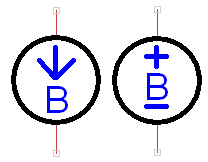
\includegraphics[width=0.15\textwidth]{./pics/SpiceEl/BSource.png}
  \end{center}
\end{figure}

\textbf{\textit{Schematics Editor Option:}}

"\textsf{I/V}" used to describe the current/voltage of the source with an expression \texttt{[I/V]}

\inserttip{One can define the Current OR the voltage of a behavioral source but not both!}

\textbf{\textit{Examples:}}

\begin{longtable}{l l}
%\textit{statement} & \textit{explanation} \\ [0.5ex]
Statement & Explanation \\ [0.5ex]
\hline \\ %\vspace{-0.8\parskip} 

\begin{minipage}{15em}
\texttt{B1 0 1 I=cos(v(1))+sin(v(2))}
\end{minipage}& 
\begin{minipage}{20em}
Insert current source B1, with current equal to the expression cos(v(1))+sin(v(2))
\end{minipage}
\\ \\

\begin{minipage}{15em}
B2 0 1 V=ln(cos(log(v(1,2)\^{}2)))-v(2)\^{}v(1)
\end{minipage} &
\begin{minipage}{20em}
Insert voltage source B2, with voltage equal to the expression V=ln(cos(log(v(1,2)$\rm{^2}$)))-v(2)$\rm{^{v(1)}}$
\end{minipage}
\\ \\

\begin{minipage}{15em}
B3 0 1 V=V(1) $<$ $\left\{\rm{Vlow}\right\}$ ? $\left\{\rm{Vlow}\right\}$ : V(1) $>$ $\left\{\rm{Vhigh}\right\}$ ? $\left\{\rm{Vhigh}\right\}$ : V(1)
\end{minipage} &
\begin{minipage}{20em}
Insert voltage source B3, with voltage equal to the voltage of net/node 1 bounded by parameters 'Vlow' and 'Vhigh'
\end{minipage}
\\ \\

\begin{minipage}{15em}
Bfib 0 1 V=pwl({time}, 0,1, 1,1, 2,2, 3,3, 4,5, 5,8, 6,13, 7,21)
\end{minipage} &
\begin{minipage}{20em}
Insert voltage source Bfib, with voltage equal to the Fibonacci series as a function of time.
\end{minipage}

\end{longtable}

\textbf{\textit{Available functions for behavioral sources:}}

\begin{longtable}{c c}

\hline\hline %inserts double horizontal lines
Function Name & Description \\ [0.5ex] % inserts table
%heading
\hline % inserts single horizontal line
abs(x) & Absolute value of x \\ \\ % inserting body of the table

absdelay(x, del), delay(x, del) & \begin{minipage}{20em}
Value of x del amount of independent units before the current value of the independent variable. If the independent variable is less than the delay parameter del zero.
\end{minipage}\\ \\

arcsin(x), asin(x), arccos(x),\\ 
acos(x), arctan(x), atan(x) & \begin{minipage}{20em}
Inverse trigonometric functions. Note these functions give the real part only.
\end{minipage}\\ \\

asinh(x), acosh(x), atanh(x) & \begin{minipage}{20em}
Inverse hyperbolic trigonometric functions. Note these functions give the real part only.
\end{minipage}\\ \\

atan2(y, x) & \begin{minipage}{20em}
Fourth quadrant inverse tangent of y$/$x
\end{minipage}\\ \\

buf(x) & \begin{minipage}{20em}
(x$>$0.5) ? 1.0 : 0.0
\end{minipage}\\ \\

ceil(x) & \begin{minipage}{20em}
Smallest integer that is greater than or equal to x
\end{minipage}\\ \\

ddt(x) & \begin{minipage}{20em}
derivative of x against the independent variable
\end{minipage}\\ \\

exp(x) & \begin{minipage}{20em}
e$\rm{^x}$
\end{minipage}\\ \\

floor(x), int(x) & \begin{minipage}{20em}
Largest integer that is less than or equal to x
\end{minipage}\\ \\

hypot(x, y) & \begin{minipage}{20em}
sqrt((x$\rm{^2}$) + (y$\rm{^2}$))
\end{minipage}\\ \\

idt(x[,o[,r]]), sdt(x[,o[r]]) & \begin{minipage}{20em}
Integral of x against the independent variable. 'o' is an optional offset parameter. 'r' is an option reset parameter. If 'r' is true the integral resets to 'o'.
\end{minipage}\\ \\

inv(x) & \begin{minipage}{20em}
(x$>$0.5) ? 0.0 : 1.0
\end{minipage}\\ \\

limit(x, y, z) & \begin{minipage}{20em}
If y $\leq$ x then x, If x $<$ y $<$ z then y, if x $<$ y and z $\leq$ y then z.  
\end{minipage}\\ \\

ln(x), log(x) & \begin{minipage}{20em}
Natural log of absolute value of x, causes error if x is zero
\end{minipage}\\ \\

log10(x) & \begin{minipage}{20em}
Log base ten of absolute value of x, causes error if x is zero
\end{minipage}\\ \\

max(x, y) & \begin{minipage}{20em}
x $>$ y ? x : y
\end{minipage}\\ \\

min(x, y) & \begin{minipage}{20em}
x $<$ y ? x : y
\end{minipage}\\ \\

pow(x, y) & \begin{minipage}{20em}
x raised to the power of y (pow from C runtime library)
\end{minipage}\\ \\

pwr(x, y) & \begin{minipage}{20em}
pow(fabs(x),y), note that this function gives only the real part of the answer
\end{minipage}\\ \\

pwrs(x, y) & \begin{minipage}{20em}
sgn(x)$\cdot$abs(x)$\rm{^y}$
\end{minipage}\\ \\

pwl(x, $\rm{x_1,y_1, x_2,y_2}$...) & \begin{minipage}{20em}
Piecewise linear function where the answer value y, is interpolated base on the pair of points between which x falls. Note that the x values of the points must increase monotonically.
\end{minipage}\\ \\

rand(x), random(x) & \begin{minipage}{20em}
Randomly generated real number y such that \\0 $<$ y $<$ 1 depending on the integer value of x
\end{minipage}\\ \\

round(x) & \begin{minipage}{20em}
Round to nearest integer, x.5 rounds up.
\end{minipage}\\ \\

sgn(x) & \begin{minipage}{20em}
1.0 for x $>$ 0, 0.0 for x equal to 0, -1.0 for x $<$ 0 
\end{minipage}\\ \\

sin(x), cos(x), tan(x) & \begin{minipage}{20em}
Trigonometric functions
\end{minipage}\\ \\

sinh(x), cosh(x), tanh(x) & \begin{minipage}{20em}
Hyperbolic trigonometric functions
\end{minipage}\\ \\

sqrt(x) & \begin{minipage}{20em}
y=$\sqrt{\rm{x}}$, note that if x is less than zero this function returns the square root of the absolute value of x
\end{minipage}\\ \\

%table(x, x1,y1, x2,y2, ... ) & \begin{minipage}{20em}
%Piecewise linear function where the answer value y, is interpolated base on the pair of points between which x falls.
%\end{minipage}\\ \\

ternary\_fcn(x, y, z), if(x, y, z), x ? y : z & \begin{minipage}{20em}
x ? y : z, (read as "if x then y else z") note the question mark must be followed by a blank space for the parser
\end{minipage}\\ \\

u(x) & \begin{minipage}{20em}
Unit step, x $>$ 0 ? 1 : 0
\end{minipage}\\ \\

unif(nom, rvar) & \begin{minipage}{20em}
Nominal value plus relative variation (to nominal) uniformly distributed between $\pm$rvar
\end{minipage}\\ \\

uramp(x) & \begin{minipage}{20em}
x $>$ 0 ? x : 0
\end{minipage}\\ \\

white(x) & \begin{minipage}{20em}
Randomly generated number y such that -0.5 $<$ y $<$ 0.5
\end{minipage}\\ \\[1ex] % [1ex] adds vertical space
\hline %inserts single line

\caption{Behavioral source functions}
\label {tab:paramfuncs}
\end{longtable}

\textbf{\textit{Available logical operators for behavioral sources: $!=, <>, >=, <=, ==, >, <, ||, \&\&, !$ }}

\subsection{Special Behavioral Source Variables time, temper, temp, hertz}
\textbf{\textit{'time', 'temper' and 'temp' are available in transient for the simulation time and temperature. For example "B1 1 0 v=sin($\rm{\left\{time\right\}}$)" produces a sinusoidal voltage source. 'hertz' is available in AC analyses but may slow the simulation.}}

\newpage
\section{Active Elements}
\label{sec_sceadm_activeelements}

\subsection{Diodes}
\label{subsec_sceadm_diodes}

\subsection{BJTs}
\label{subsec_sceadm_bjts}

\subsection{MOSFETs}
\label{subsec_sceadm_mosfets}

\subsection{Other Active Elements}
\label{subsec_sceadm_otheractiveelements}

\textbf{\textit{JFETs}}


\textbf{\textit{MESFETs}}



\section{Other Elements}
\label{sec_sceadm_otherelements}

\subsection{Switches}
\label{subsec_sceadm_switches}

\subsection{Transmission Lines}
\label{subsec_sceadm_transmissionlines}

\section{Built-in Subcircuits and Behavioral Elements in CoolSPICE}
\label{sec_sceadm_builtinsubcircuits}

\subsection{Probes}
\label{subsec_sceadm_probes}

Probes, which are found in the \textsf{Analog} library of CoolSPICE, are described in detail in Section \ref{subsec_satco_savestatement}, which is about their associated \texttt{.save} statement.  

\subsection{The \texttt{.include} Statement}
\label{sec_sceadm_includestatement}

\subsection{The \texttt{.subckt} Statement and Subcircuit Definition}
\label{sec_sceadm_subcktstatement}

